
\begin{figure}[t]
    \centering
    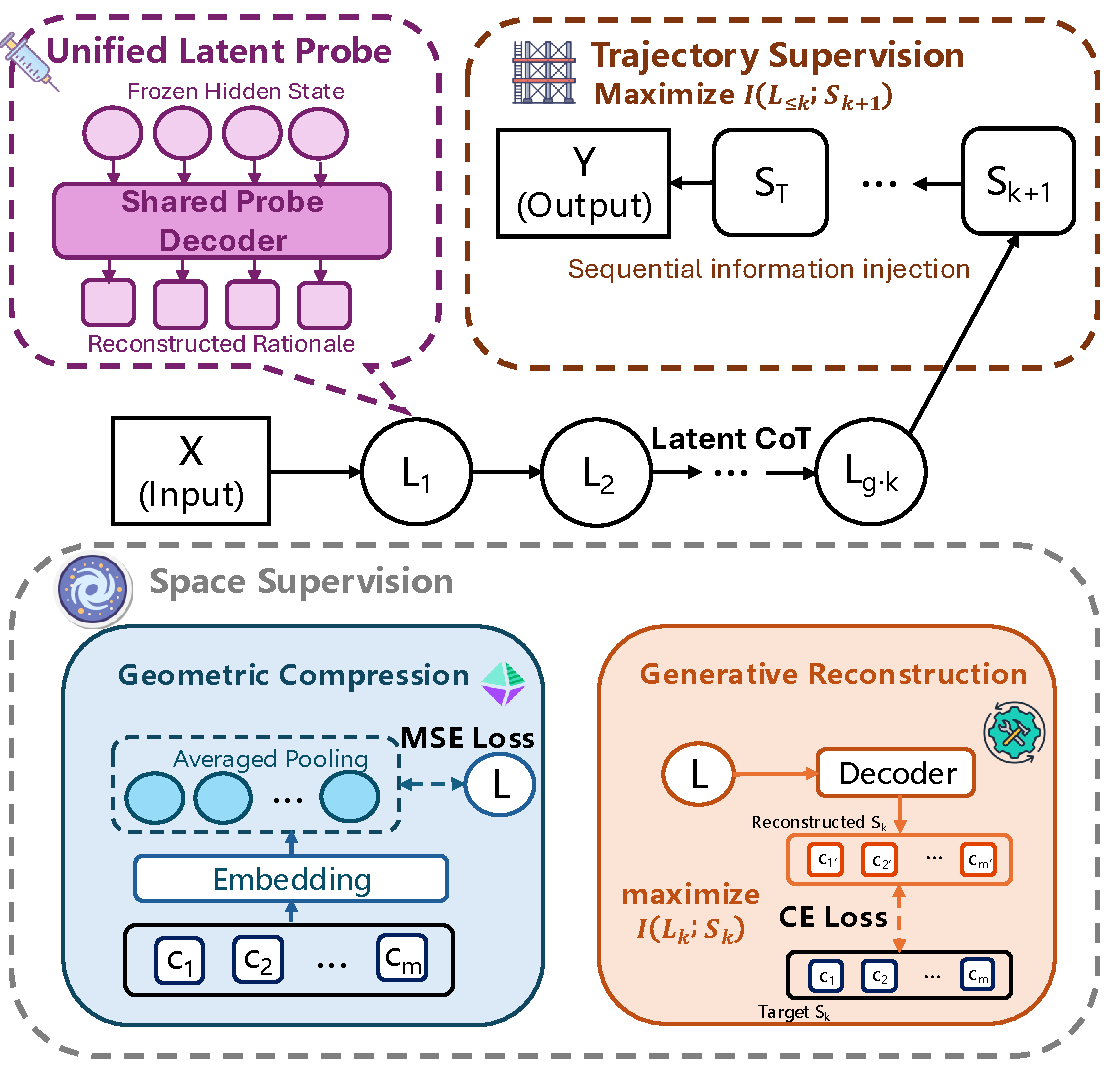
\includegraphics[width=\linewidth]{Figures/figure-1.pdf}
    \caption{
    Overview of our information-theoretic framework for Latent CoT. Process supervision is decomposed into trajectory supervision for sequential information injection and space supervision for semantic anchoring, while ULP probes frozen latent states to quantify recoverable reasoning information.
    }
    \label{fig:overview}
\end{figure}


\section{Introduction}
\label{sec:intro}

Large Language Models (LLMs) have achieved strong performance on complex reasoning tasks by generating explicit chain-of-thought (CoT) sequences~\citep{wei2022chain, Guo2025DeepSeekR1, chen2025reasoning}. However, representing reasoning as verbose sequences of natural language introduces intrinsic constraints. First, explicit CoT suffers from expressive redundancy: many tokens in a reasoning chain are syntactically necessary but functionally irrelevant, leading to inflated sequence lengths without proportional gains in reasoning quality~\citep{feng2025efficient, li2025implicitreasoninglargelanguage}. Second, it imposes a semantic bottleneck: as abstract, continuous, and compositional reasoning processes cannot be faithfully represented within natural language space, inevitably causing information loss~\citep{chen2025reasoninglanguagecomprehensivesurvey, reasoningdark, Sun2025LatentCF}. These limitations have motivated Latent Chain-of-Thought, which internalizes reasoning within continuous hidden states rather than externalizing it as text~\citep{hao2025training, shen-etal-2025-codi}. By removing the low-bandwidth constraint of discrete tokens, latent CoT enables a more expressive and computationally efficient form of internalized ``System 2'' reasoning~\citep{deng2024explicitcotimplicitcot,geiping2025scaling}.

Despite its promise, achieving robust latent CoT remains challenging~\citep{lindsey2025biology, simcot}. A central difficulty lies in the representation shift from the discrete text space used in pre-training to high-dimensional continuous latent spaces, which requires models to adapt to a fundamentally different regime. Furthermore, this latent space is not directly interpretable, making it difficult to provide explicit supervision~\citep{chen-etal-2025-unveiling-key,colar,pttslatent}. While a growing body of work has introduced additional supervision strategies to stabilize training~\citep{hao2025training, shen-etal-2025-codi, butt2025softtokenshardtruths, deng2026llmlatentreasoningchain, li2026dynamicslatentchainofthoughtempirical}, the field lacks a principled framework for understanding how these signals govern the geometry and dynamics of the latent reasoning space.


To bridge this gap, we formalize Latent CoT through an information-theoretic lens. We begin by examining the most intuitive baseline: outcome supervision, which attempts to directly maximize the mutual information between latent reasoning steps and the final answer. Empirically, this approach performs no better than standard non-CoT baselines. We trace this failure to a dual collapse. From an optimization standpoint, it suffers from gradient attenuation; the sparse outcome signal decays so rapidly across the latent trajectory that credit assignment fails. From a representational standpoint, the latent manifold progressively drifts away from the semantic structure of the token space, indicating that \emph{outcome supervision alone is insufficient to induce meaningful latent CoT steps}.


Given the dual collapse of outcome supervision, we review the fragmented landscape of existing Latent CoT research and identify a broader family of \textbf{process supervision} methods, which use explicit rationales to provide intermediate guidance beyond the final answer. 
We deconstruct process supervision into two conceptually distinct but interacting dimensions: \textit{trajectory supervision} and \textit{space supervision}.
Figure~\ref{fig:overview} provides an overview of this framework.

Trajectory supervision addresses the temporal decay of information by providing dense, stepwise signals, training latent states to predict ``suffixes'' of explicit reasoning sequences. This acts as a mechanism for sequential information injection, effectively maximizing the mutual information between current latent steps and future reasoning trajectories. Space supervision, conversely, manages the structural integrity of the manifold itself by anchoring it to a known semantic domain. This is achieved either through geometric compression, which forces latent states into a rigid alignment with token embeddings, or generative reconstruction, which requires the states to remain decodable into natural language. Both approaches attempt to maximize mutual information between latent states and corresponding CoT steps, but with different inductive biases.

Our empirical analysis reveals a delicate interplay between these dimensions. Process supervision significantly stabilizes training. We observe that inserting new latent steps leads to increased gradient magnitudes, indicating active adaptation rather than attenuation. Furthermore, we find that optimizer resetting is crucial for inducing effective training signals at each stage, preventing interference between newly introduced latent variables and previously learned representations. The effectiveness of space supervision signals, however, is highly dependent on the nature of supervision applied. While geometric compression often introduces a ``destructive prior'' that collapses the reasoning manifold and reduces its information capacity, generative reconstruction acts as a flexible semantic tether. It preserves the intrinsic dimensionality of the latent space and serves as a calibration mechanism that mitigates semantic drift.

To quantify these effects, we introduce the \textbf{Unified Latent Probe (ULP)}, a variational reconstruction-based diagnostic framework that trains a shared conditional decoder to recover step-wise explicit reasoning from frozen latent hidden states extracted across models. By operationalizing mutual information as a reconstruction objective over a unified probing dataset, ULP provides a principled measure of how much structured reasoning is preserved and recoverable in continuous latent space. This reveals a clear information–performance binding: reasoning accuracy scales with the amount of information preserved in latent representations.
Our contributions are as follows:
\begin{itemize}
    \item Diagnosis of the Optimization Barrier: We demonstrate that the failure of outcome-supervised Latent CoT is an information-theoretic collapse, and that dense, sequential information injection (process supervision) is required to induce valid latent dynamics.
    \item The Unified Latent Probe (ULP): We design a rigorous diagnostic instrument that solves the ``black box'' verification problem by quantitatively linking representational fidelity (mutual information) to downstream reasoning performance.
    \item Generative Reconstruction over Geometric Compression: We establish that effective supervision must prioritize the preservation of information capacity via. e.g., generative reconstruction rather than rigid geometric compression.
\end{itemize}

